\documentclass[12pt]{article}
\usepackage{uwyo_report} % loads in all the specific formatting
\usepackage{amsmath}
\usepackage{amssymb}
\usepackage{float}


% if you want other packages, put them here

% macro for typesetting the word BibTeX
\def\BibTeX{{\rm B\kern-.05em{\sc i\kern-.025em b}\kern-.08em
   T\kern-.1667em\lower.7ex\hbox{E}\kern-.125emX}}


\begin{document}

\title{EE 5450  Project 01: Simultaneous Monocular Calibration and Pose Estimation}

\author{David R. Mohler}

%\date{December 7, 1941}

\maketitle

\section{Introduction}
The following set of experiments are focused on the application of the simultaneous monocular calibration and pose estimation algorithm to a series of images of rigid objects with known dimensions and correspondence points. This algorithm is, as described by its title, capable of calibrating a single camera with a fixed focal length in the presence of known rigid objects, which enables the simultaneous discovery of the pose of the object and from this generate a three dimensional representation of that same object.  

In this project we will demonstrate the generation of independent and identically distributed (IID) data samples through rejection sampling of a continuous PDF. Using this data we will then apply EM to iteratively estimate the parameters of the probability distribution function. 

\section{Methods and Results}
The foundation of this project is based on the known characterization of a signal which is represented in the form a single continuous PDF as seen in Equation \ref{PDF}. It is apparent from Equation \ref{PDF} that our signal is characterized as a continuous probability mixture model, consisting of three distinct mixture components. By separating these components (Figure \ref{comps}) we display the contributions of each respective distribution to the cumulative PDF.

\begin{center}
	\begin{tabular}[5pt]{| c| c|}
	\hline
    Parameter	& Value \\[0.5ex] 
	\hline 
	
	$w_1$& 0.5  \\ \hline 
	$w_2$& 0.3  \\ \hline 
	$w_3$& 0.2  \\ \hline 
	$\mu_1$& 3.0  \\ \hline 
	$\mu_2$& 10.0  \\ \hline 
	$\sigma_1^2$& 1.0  \\ \hline 
	$\sigma_2^2$& 4.0  \\ \hline 
	$\lambda$& 2.0  \\ \hline 
\end{tabular}
\captionof{table}{True Distribution Parameters}\label{truevals}
\end{center}
 Using the given values, seen in Table \ref{truevals}, we display the separated components of the probability mixture. Our mixture model is composed of two separate Gaussian distributions, each with their own respective means and variances, and a single exponential distribution which is characterized by the $\lambda$ parameter, which can be interpreted as the inverse of the mean of the exponential distribution.

%\begin{figure}[h]
%	\centering % must do this or your figure won't be centered
%	\includegraphics[width=0.5\textwidth]{comps.eps}
%	\caption{Components of the probability mixture model.} \label{comps}
%\end{figure}

\begin{equation}\label{PDF}
p(x) = w_1 \dfrac{1}{\sqrt{2\pi\sigma_{1}^{2}}}e^{-\dfrac{1}{2}\dfrac{(x-\mu_1)^2}{\sigma_{1}^{2}}}+w_2 \dfrac{1}{\sqrt{2\pi\sigma_{2}^{2}}}e^{-\dfrac{1}{2}\dfrac{(x-\mu_2)^2}{\sigma_{2}^{2}}}+w_3\lambda e^{-\lambda x}
\end{equation}
To maintain the constraint that $\int p(x) dx=1$, each mixture component is assigned a weight such that $\sum_{i} w_i = 1$. The true distribution is constructed such that $w_1 = 0.5$, $w_2 = 0.3$, and $w_3 = 0.2$. The results of the weighted mixture that constitutes the continuous distribution $p(x)$ can be seen in Figure \ref{true}.
%\begin{figure}[H]
%	\centering % must do this or your figure won't be centered
%	\includegraphics[width=0.5\textwidth]{true.eps}
%	\caption{True probability distribution} \label{true}
%\end{figure}


\subsection{Corrupted Correspondence Points}

	\begin{figure}[h]
	\centering % must do this or your figure won't be centered
	\captionsetup{justification=centering}
	\begin{minipage}{0.5\textwidth}
		\centering
		\includegraphics[width=1\textwidth]{noise_shift.eps}
		\caption{Estimated image coordinates} \label{noiseshift}
	\end{minipage}\hfill
	\begin{minipage}{0.5\textwidth}
		\centering % must do this or your figure won't be centered
		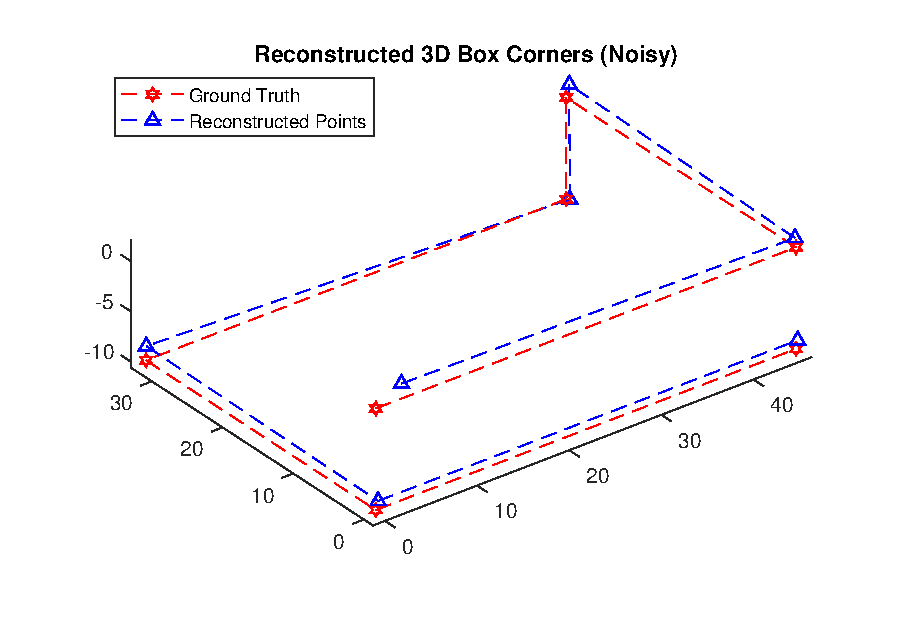
\includegraphics[width=1\textwidth]{noise_shift_recon.eps}
		\caption{Reconstructed box relative to ground truth} \label{noiserecon}
	\end{minipage}
\end{figure}

	\begin{figure}[h]
	\centering % must do this or your figure won't be centered
	\captionsetup{justification=centering}
	\begin{minipage}{0.5\textwidth}
		\centering
		\includegraphics[width=1\textwidth]{noise_all.eps}
		\caption{Estimated image coordinates \newline(unique coordinate component noise)} \label{noiseall}
	\end{minipage}\hfill
	\begin{minipage}{0.5\textwidth}
		\centering % must do this or your figure won't be centered
		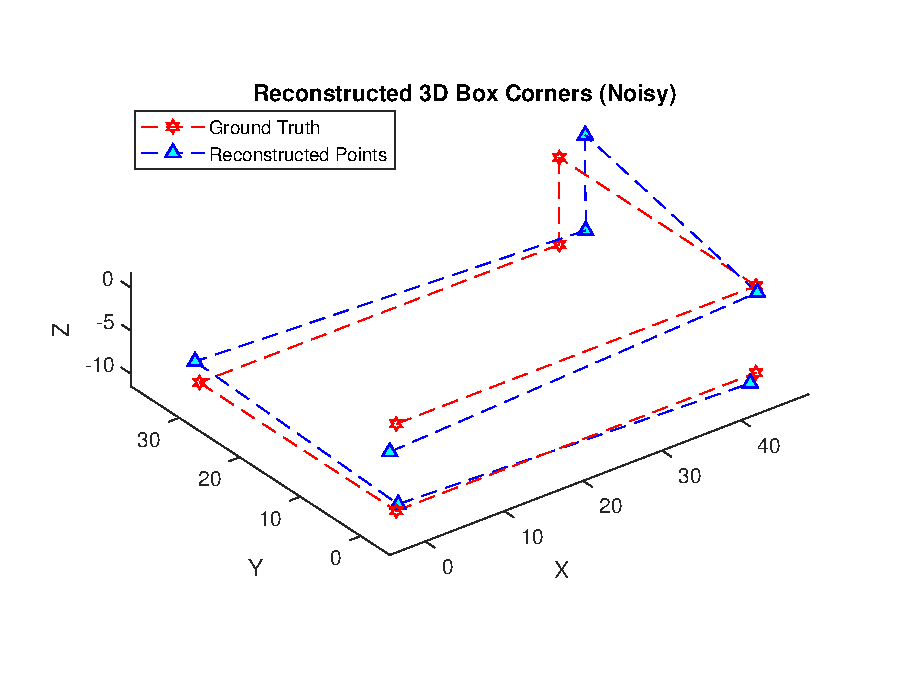
\includegraphics[width=1\textwidth]{noise_all_recon.eps}
		\caption{Reconstructed box relative to ground truth} \label{noiseallrecon}
	\end{minipage}
\end{figure}

\subsection{Improper Dimensions}



\section{Conclusions}

In this project we have demonstrated two major methods critical to estimation and uncertainty quantification. The first being a method to sample from any arbitrary closed functional form of a continuous probability distribution, and the second being the application of the Expectation Maximization algorithm to a probability mixture model. For our implementation the rejection sampling method is essential to the proper operation of the EM algorithm. Rejection sampling provides a simple method for artificial data generation. By varying the number of data points that we wish to sample from our known functional form of the distribution we are able to view the accuracy of the sampled PDF relative to the true curve. It is noted that the number of data points required to generate an ``accurate'' curve is application and computational burden dependent. For the purposes of this project we found that samples ranging in the low hundreds did not provide enough data to create a decent approximation, however, beyond 1000 samples we were able to obtain good results with low margins of error. From this, we note that balancing between excessive computation and accuracy requirements lacks a singular hard threshold and should be approached with the specific design parameters in mind.

The Expectation Maximization algorithm has proven itself to be a fairly robust tool for the approximation of distribution parameters. When provided with a sufficient number of samples and reasonable initializations of the estimated parameters EM is,on average, capable of producing results with single digit error precision (percentage).  However, it is not entirely immune to failure. The algorithm diverges in cases where it is initially assumed that the weight of any given component is zero, or the variance of any given Gaussian component is initialized with a zero value. Similarly, while not entirely failing, the margin of error that occurs in the impoverished case of too few samples provided to the algorithm is vastly larger on average. This error margin was observed to reach a mean of as high as nearly $41\%$ error, roughly 8 times as large as that of the trials performed with a sufficient number of samples. We have also demonstrated that the algorithm tends to provide better performance when faced with distributions that are, for the most part distinct and separate. Whereas when tasked with a distribution that is heavily mixed and the components are largely indistinguishable from one another, the performance is much poorer, even with strong initialization parameters.



\appendix % this command sets sectioning command to the appendix format
% uncomment the next line to start on a fresh page
\newpage

\section{Code Listings}\label{code}

% input the file containing the code
\lstinputlisting[caption={Top level implementation for Monocular Calibration and Pose Estimation},label={proj}]{MonoPose.m}
\lstinputlisting[caption={QR Decomp Based Algorithm Implementation},label={alg}]{MonoPoseQR.m} 
\lstinputlisting[caption={Rearranged QR Decomposition (Credit: Dr. John McInroy)},label={qrCom}]{qrCommute.m}
%\lstinputlisting[caption={Expectation Maximization, Version 2},label={EM2}]{EM2.m}
%\lstinputlisting[caption={Mixture Model PDF},label={prob}]{p.m}


%% The commands below automatically generate the References section
%% using the ``sample_bib'' file I've given you.

\newpage  % start a new page

\bibliographystyle{ieeetr}
\bibliography{a1_abbrv,Proj2}

\end{document} % always the last line of your document file
